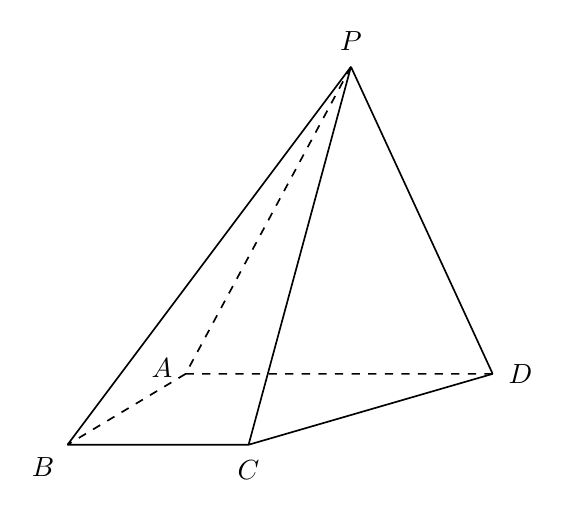
\begin{tikzpicture}[line width=0.6pt, font=\normalsize]
\tikzset{hid/.style={dashed}, lbl/.style={font=\normalsize, fill=white, inner sep=1.5pt}}
\coordinate (B) at (0,0); \coordinate (C) at (2.3,0); \coordinate (D) at (5.4,0.9); \coordinate (A) at (1.5,0.9);
\coordinate (P) at (3.6,4.8);
\draw (B)--(C)--(D);
\draw[hid] (D)--(A) (A)--(B);
\draw (P)--(B) (P)--(C) (P)--(D);
\draw[hid] (P)--(A);
\node[lbl, above=4pt] at (P) {$P$};
\node[lbl, below left=3pt] at (B) {$B$};
\node[lbl, below=4pt] at (C) {$C$};
\node[lbl, right=4pt] at (D) {$D$};
\node[lbl, left=3pt,fill=none,xshift=0.00bp,yshift=2.00bp] at (A) {$A$};
\end{tikzpicture}
